% !TEX root = ../../prj4projektrapport.tex
% SKAL STÅ I TOPPEN AF ALLE FILER FOR AT MASTER-filen KOMPILERES 


\section{Brugergrænseflade}

Brugergrænsefladen i dette projekt er designet på en HMI KTP 600. Den kan tilgåes gennem en switch af typen CSM 1277. I dette afsnit vil overvejelser omkring HMI'et blive gennemgået, koden og opsætningen er froklaret i dokumentationen.\footnote{Projektdokumentationen, 10.2, Brugergrænseflade}


Systemet der udvikles skulle være operatørvenligt, hvilket har været grundlag for mange beslutninger omkring HMI'et. Det skal være let at gennemskue og der skal kun være de mest nødvendigt funktionaliteter, for at give overblik.
Der er derfor fremstillet to skærme; automatisk mode og manuel mode. Der er få forskelle på de to, men det tydeliggør for operatøren, hvilken tilstand der er aktiv. Skærmen for automatisk mode kan ses på figur \ref{fig:HMIAutomatiskModeDesign}. Skærmen for manuel mode kan findes i dokumentationen.\footnote{Projektdokumentationen, 10.2.2, Manuel mode}

\begin{figure}[H] % (alternativt [H])
	\centering
	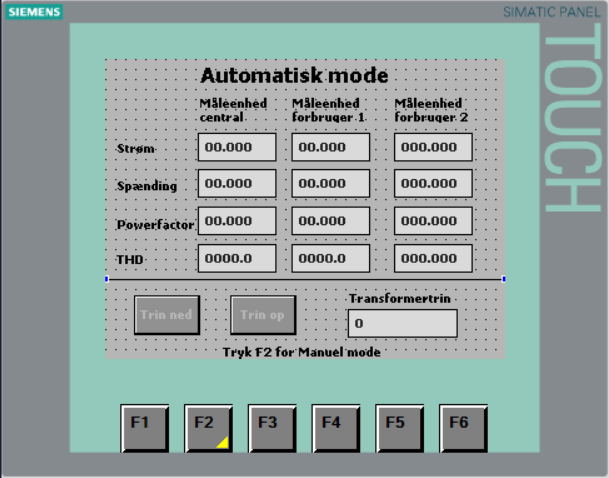
\includegraphics[width=0.7\textwidth]{Figure/HMIAutomatiskModeDesign}
	\caption{HMI i automatisk mode}
	\label{fig:HMIAutomatiskModeDesign}
\end{figure}

På begge skærme vises data for Måleenhederne i kolonner og rækker, for at give overblik. En mangel her er at det ikke er vist hvilken enhed, dataet vises i. For spænding er det i volt, strøm i ampere, power factor er enhedsløs og THD er vises som det samlede indhold af frekvenser i procent af den fundamentale frekvens. THD er forklaret i afsnit !!REFERENCE THD!!!.


Under skillelinjen ses al information omkring Trinskifteren. I automatisk mode er det ikke muligt at skifte trin på knapperne Trin ned og Trin op, derfor er de gråskalerede. I manuel mode er de sort/hvid for at vise at de kan benyttes.


Knappen til tilstandsskift er på hver skærm placeret på F-knapperne med tilhørende forklarende tekst på skærmen, for at tydeliggør funktonaliteten af knapperne.


Systemet er klargjort til at en central og to decentrale Måleenheder, men i det endelige produkt er kun en central og en decentral Måleenhed. Forbruger 2 er derfor ikke aktiv i produktet.